\documentclass[11pt]{amsart}
\usepackage[margin=.75in]{geometry} 
\usepackage[parfill]{parskip}%\usepackage{graphicx}
\usepackage{graphicx}
%SetFonts
% libertine text and newtxmath
\usepackage{libertine}
\usepackage[TS1,T1]{fontenc}
\usepackage{textcomp}
\usepackage[scaled=.85]{beramono} 
\usepackage[libertine,cmbraces]{newtxmath}
\makeatletter
\def\libertine@figurestyle{OsF}
\makeatother
%\def\libertine{\fontfamily{fxlj}\selectfont}
%SetFonts
\usepackage[supstfm=libertinesups,%
  supscaled=1.2,%
  raised=-.13em]{superiors}
\title{Superior Figures}
\author{Michael Sharpe}
\date{\today}  % Activate to display a given date or no date

\begin{document}
\maketitle
\section{Briefly}
The default behavior of footnote and endnote markers in \LaTeX\ is to print the number as if it were a mathematical superscript. In most cases, this means the size is about 70\% of the normal lining figure and the top is somewhat above the tops of capital letters. In many cases, the superscript figure is simply reduced in all dimensions by about 70\%, making them appear rather slight, though overly tall. (The \textsf{libertine} package used for preparing this document has a custom footnote illustrated below.)

As an alternative, one may use superior figures---small figures, usually 50\% to 60\% of the height of lining figures, like \textsu{1234567890}. Commonly, they are designed so that the tops of the numbers are aligned with the tops of the capital letters in the font, though sometimes a little higher, corresponding to the ascender height. PostScript fonts have for a long time mostly contained just a small subset $\{1,2,3\}$ of the possible superior digits, and most OpenType fonts in the Adobe portfolio, other than the most popular and the most recent, contain the same small subset. Moreover, the \textsf{TS1} encoding includes slots for only those three superior figures. Even the recent STIX collection contains just the basic three.


This package allows you to add a full set of superior figures to a font family that lacks one. It uses two predefined collections---the default is {\tt ntxsups}, a collection matching Times, derived from the STIX fonts (digits 1..8 were taken from the vulgar fraction glyphs, and the digits 0, 9 were constructed to match them using FontForge) while the second, {\tt libertinesups}, is taken from Libertine-Legacy. (The standard \textsf{libertine} package provides no access to these glyphs other than through footnote markers.) In addition, you may specify any \TeX\ tfm whose figure slots contain superior figures. The package also allows you to scale the size of the imported figures, to take into account your general font scaling,  and to specify an amount by which to raise the imported, rescaled figures. You may also specify a spacing to apply before the footnote marker, using the parameter {\tt supspaced}. The package should be loaded after your Roman text font package\footnote{The {\tt newtxtext} package uses the {\tt ntxsups} superiors contained in the newtx package by default for footnote markers.}. 

\textsc{Sample Invocations:}

\begin{itemize}
\item Times-like, no rescaling or raising, but with $.04${\tt em} space before footnote markers:
\begin{verbatim}
\usepackage[supspaced=.04em]{superiors}
\end{verbatim}
\item Libertine superiors scaled up by 20\%, then lowered:
\begin{verbatim}
\usepackage{libertine}
\usepackage[supstfm=libertinesups,%
  supscaled=1.2,%
  raised=-.13em]% match XHeight of libertine
{superiors}
\end{verbatim}
\item Use MinionPro\footnote{Assumes you have installed MinionPro according to the directions in the \textsf{minion2newtx} package.}
 superiors at default size, lowered a bit:
\begin{verbatim}
\usepackage[supstfm=T1-Minion2Pro-Regular-sups-kern-liga,%
  raised=-.05em]%
{superiors}
\end{verbatim}
\end{itemize}

It is best to specify a relative unit for the {\tt raised} and {\tt supspaced} parameters so that they change with the font size. (Recall that for a $10${\tt pt} font, {\tt 1em} is usually {\tt 10pt}, but the actual size of {\tt 1em} is defined relative to font size.)

The following example compares libertine with its default footnote markers against libertine with the superiors package as described in the second example above:

\[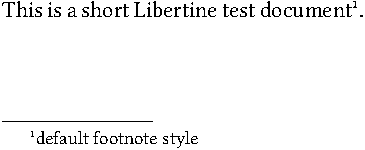
\includegraphics{libfoot0-crop} \qquad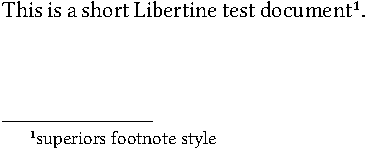
\includegraphics{libfoot1-crop}\]

There is another parameter named {\tt scaled} that should be used only if you loaded your text font with a scale parameter different from $1.0$, and in this case, you should use the same scale parameter. For example:
\begin{verbatim}
\usepackage[lining,scaled=1.05]{bembo}
\usepackage[scaled=1.05,%
  supstfm=libertinesups,% libertine
  supscaled=1.2,%
  raised=-.13em]%
{superiors}
\end{verbatim}
\section{Issues with superior figures}
If a number of figure styles are available, many packages make use of \textsf{nfssext} (or its further extension \textsf{nfssext-cfr}) to access those special forms. For superior figures, two macros are defined by \textsf{nfssext}: \verb|\sustyle| and \verb|\textsu|, the first of which changes the text font to a font with superior figures (and is usually called with action confined to a group), while the second is a macro called like \verb|\textsu{123}| which applies \verb|\sustyle| to just its argument. In packages generated by {\tt otfinst}, if superior figures are available (even if only three of them), it redefines \verb|\@makefnmark|:
\begin{verbatim}
\def\@makefnmark{\hbox{\sustyle\@thefnmark}}
\end{verbatim}
so that it uses figures in \verb|\sustyle|. That leads to problems if you use footnote markers greater than three. For example, in Stempel Garamond, where there are only three superior figures available, the first graphic shows the default footnote markers provided by \textsf{otfinst}, the second shows the document processed with libertine footnote markers using 
\begin{verbatim}
\usepackage[supstfm=libertinesups,%
  supscaled=1.2,%
  raised=-.04em
]{superiors}
\end{verbatim}

\[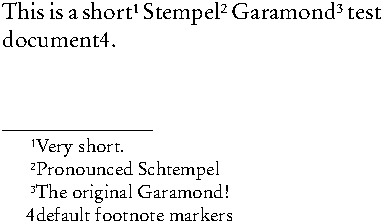
\includegraphics{stempelfoot0-crop} \qquad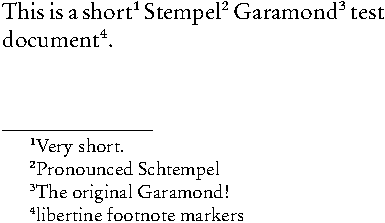
\includegraphics{stempelfoot1-crop}\]
This package redefines these macros so that \verb|\sustyle| changes the font and applies the scaling changes, while changes due to the {\tt raised} parameter are applied only within \verb|\textsu|. For this reason, we have to modify the definition of \verb|\@makefnmark| as follows:
\begin{verbatim}
\def\@makefnmark{\hbox{\textsu{\hspace*{superiors@spaced}\@thefnmark}}}
\end{verbatim}

Relatively few Opentype text font families have a complete set of superior figures that can be accessed after running \textsf{otfinst}. Other than those listed above, the following are known to me to have a complete set of superior figures:
\begin{verbatim}
Adobe Bembo Std
Adobe Caslon Pro
Adobe Warnock Pro
Monotype Dante Std
Monotype Bell Std
Monotype Perpetua Std
Adobe Garamond Premier Pro
Adobe Brioso Pro
Adobe Arno Pro
Adobe Kinesis Std
Adobe Jenson Pro
Adobe Kepler Std
\end{verbatim}

\end{document}  